%!TeX encoding = UTF-8
%!TeX program = xelatex

\documentclass[notheorems, aspectratio=169, mathserif]{beamer}
% aspectratio: 1610, 149, 54, 43(default), 32

% Input configuration
\usepackage[utf8]{inputenc}

% -- support vietnamese --
% \usepackage[vietnamese]{babel}
% -- support english --
\usepackage[english]{babel}
% ----------------------------------------------

% For math
\usepackage{amsmath,amssymb}
\usepackage{mathtools}
\usepackage{amsthm}
\newcommand{\N}{\mathbb{N}}
\newcommand{\Z}{\mathbb{Z}}
\newcommand{\R}{\mathbb{R}}
\newcommand{\F}{\mathbb{F}}
% ----------------------------------------------

% For images, colors
\usepackage{graphicx}
\usepackage{color,xcolor}
% ----------------------------------------------

% For captioning
\usepackage{caption}
\setbeamertemplate{caption}[numbered]
% ----------------------------------------------

% For tables
\usepackage{booktabs}
% ----------------------------------------------

% For hyper references between sections
\usepackage{hyperref}
% ----------------------------------------------

% For texts, algorithm and codes
\usepackage{ulem}
\usepackage{algorithm}
\usepackage{listings}
% ----------------------------------------------

% For tikz
\usepackage{framed}
\usepackage{tikz}
\usepackage{pgf}
\usetikzlibrary{calc,trees,positioning,arrows,chains,shapes.geometric,%
decorations.pathreplacing,decorations.pathmorphing,shapes,%
matrix,shapes.symbols}
\pgfmathsetseed{1} % To have predictable results
% Define a background layer, in which the parchment shape is drawn
\definecolor{doge}{HTML}{0065BD}
\pgfdeclarelayer{background}
\pgfsetlayers{background, main}

% Macro to draw the shape behind the text, when it fits completly in the page
% define styles for the normal border and the torn border
\tikzset{
  normal border/.style={doge!40!black!10, decorate, 
     decoration={random steps, segment length=2.5cm, amplitude=.7mm}},
  torn border/.style={doge!40!black!5, decorate, 
     decoration={random steps, segment length=.5cm, amplitude=1.7mm}}}

% Macro to draw the shape behind the text, when it fits completly in the
% page
\def\parchmentframe#1{
\tikz{
  \node[inner sep=2em] (A) {#1};  % Draw the text of the node
  \begin{pgfonlayer}{background}  % Draw the shape behind
  \fill[normal border] 
        (A.south east) -- (A.south west) -- 
        (A.north west) -- (A.north east) -- cycle;
  \end{pgfonlayer}}}

% Macro to draw the shape, when the text will continue in next page
\def\parchmentframetop#1{
\tikz{
  \node[inner sep=2em] (A) {#1};    % Draw the text of the node
  \begin{pgfonlayer}{background}    
  \fill[normal border]              % Draw the ``complete shape'' behind
        (A.south east) -- (A.south west) -- 
        (A.north west) -- (A.north east) -- cycle;
  \fill[torn border]                % Add the torn lower border
        ($(A.south east)-(0,.2)$) -- ($(A.south west)-(0,.2)$) -- 
        ($(A.south west)+(0,.2)$) -- ($(A.south east)+(0,.2)$) -- cycle;
  \end{pgfonlayer}}}

% Macro to draw the shape, when the text continues from previous page
\def\parchmentframebottom#1{
\tikz{
  \node[inner sep=2em] (A) {#1};   % Draw the text of the node
  \begin{pgfonlayer}{background}   
  \fill[normal border]             % Draw the ``complete shape'' behind
        (A.south east) -- (A.south west) -- 
        (A.north west) -- (A.north east) -- cycle;
  \fill[torn border]               % Add the torn upper border
        ($(A.north east)-(0,.2)$) -- ($(A.north west)-(0,.2)$) -- 
        ($(A.north west)+(0,.2)$) -- ($(A.north east)+(0,.2)$) -- cycle;
  \end{pgfonlayer}}}

% Macro to draw the shape, when both the text continues from previous page
% and it will continue in next page
\def\parchmentframemiddle#1{
\tikz{
  \node[inner sep=2em] (A) {#1};   % Draw the text of the node
  \begin{pgfonlayer}{background}   
  \fill[normal border]             % Draw the ``complete shape'' behind
        (A.south east) -- (A.south west) -- 
        (A.north west) -- (A.north east) -- cycle;
  \fill[torn border]               % Add the torn lower border
        ($(A.south east)-(0,.2)$) -- ($(A.south west)-(0,.2)$) -- 
        ($(A.south west)+(0,.2)$) -- ($(A.south east)+(0,.2)$) -- cycle;
  \fill[torn border]               % Add the torn upper border
        ($(A.north east)-(0,.2)$) -- ($(A.north west)-(0,.2)$) -- 
        ($(A.north west)+(0,.2)$) -- ($(A.north east)+(0,.2)$) -- cycle;
  \end{pgfonlayer}}}

\newenvironment{parchment}[1][Example]{%
  \def\FrameCommand{\parchmentframe}%
  \def\FirstFrameCommand{\parchmentframetop}%
  \def\LastFrameCommand{\parchmentframebottom}%
  \def\MidFrameCommand{\parchmentframemiddle}%
  \vskip\baselineskip
  \MakeFramed {\FrameRestore}
  \noindent\tikz\node[inner sep=1ex, draw=white,fill=doge!30, 
          anchor=west, overlay] at (0em, 2em) {\sffamily#1};\par}%
{\endMakeFramed}
% ----------------------------------------------

% Beamer theme configuration
\mode<presentation>{
    \usetheme{default}
    % Boadilla CambridgeUS
    % default Antibes Berlin Copenhagen
    % Madrid Montpelier Ilmenau Malmoe
    % Berkeley Singapore Warsaw
    % \usecolortheme{doge}
    % beetle, beaver, orchid, whale, dolphin
    \useoutertheme{infolines}
    % infolines miniframes shadow sidebar smoothbars smoothtree split tree
    \useinnertheme{circles}
    % circles, rectanges, rounded, inmargin
}

\setbeamertemplate{blocks}[rounded][shadow]
\setbeamercolor{block title}{bg=doge!40,fg=white}
\newcommand{\reditem}[1]{\setbeamercolor{item}{fg=red}\item #1}
\newcommand*{\Scale}[2][4]{\scalebox{#1}{\ensuremath{#2}}}
\renewcommand\textbullet{\ensuremath{\bullet}}
% ----------------------------------------------

% For flow chart and codes
% Flow chart settings
\tikzset{
    >=stealth',
    punktchain/.style={
        rectangle, 
        rounded corners, 
        % fill=black!10,
        draw=white, very thick,
        text width=6em,
        minimum height=2em, 
        text centered, 
        on chain
    },
    largepunktchain/.style={
        rectangle,
        rounded corners,
        draw=white, very thick,
        text width=10em,
        minimum height=2em,
        on chain
    },
    line/.style={draw, thick, <-},
    element/.style={
        tape,
        top color=white,
        bottom color=blue!50!black!60!,
        minimum width=6em,
        draw=blue!40!black!90, very thick,
        text width=6em, 
        minimum height=2em, 
        text centered, 
        on chain
    },
    every join/.style={->, thick,shorten >=1pt},
    decoration={brace},
    tuborg/.style={decorate},
    tubnode/.style={midway, right=2pt},
    font={\fontsize{10pt}{12}\selectfont},
}

% code settings
\lstset{
    language=C++,
    basicstyle=\ttfamily\footnotesize,
    keywordstyle=\color{red},
    breaklines=true,
    xleftmargin=2em,
    numbers=left,
    numberstyle=\color[RGB]{222,155,81},
    frame=leftline,
    tabsize=4,
    breakatwhitespace=false,
    showspaces=false,               
    showstringspaces=false,
    showtabs=false,
    morekeywords={Str, Num, List},
}
% ---------------------------------------------------------------------
% title page
\makeatletter
\newcommand\titlegraphicii[1]{\def\inserttitlegraphicii{#1}}
\titlegraphicii{}
\setbeamertemplate{title page}
{
    \vskip-0.5cm%
  \vbox{}
   {\usebeamercolor[fg]{titlegraphic}\inserttitlegraphic\hfill\inserttitlegraphicii\par}
  \begin{centering}
    \begin{beamercolorbox}[sep=8pt,center]{title}
      \usebeamerfont{title}\inserttitle\par%
      \vskip0.5em
      \ifx\insertsubtitle\@empty%
      \else%
        \vskip0.25em%
        {\usebeamerfont{subtitle}\usebeamercolor[fg]{subtitle}\insertsubtitle\par}%
      \fi%     
    \end{beamercolorbox}%
    \begin{beamercolorbox}[sep=8pt,center]{author}
      \usebeamerfont{author}\insertauthor
    \end{beamercolorbox}\vskip0.5em
    \begin{beamercolorbox}[sep=8pt,center]{institute}
      \usebeamerfont{institute}\insertinstitute
    \end{beamercolorbox}
    \vskip1em\par
    \begin{beamercolorbox}[sep=8pt,center]{date}
      \usebeamerfont{date}\insertdate
    \end{beamercolorbox}%
  \end{centering}
  %\vfill
}

\makeatother
\author{Presented by Author}
\title{Presentation Title}
\subtitle{Presentation Subtile}
\institute{Department \\ University}
\date{\today}

% frame title
% https://tex.stackexchange.com/questions/231554/set-beamercolorbox-height-automatically-to-sister-beamercolorbox-on-frametitle
\makeatletter
\setbeamertemplate{frametitle}{%
    \setbeamercolor{frametitle}{bg=doge, fg=white}
    \nointerlineskip%
    \usebeamerfont{headline}%
    \nointerlineskip%
    \hbox{\hspace{-0.09\paperwidth}%
    \begin{beamercolorbox}[wd=0.1\paperwidth,vmode]{secsubsec}%
        \newdimen\titleheight%
        \setbox0=\hbox{\usebeamerfont*{frametitle}\insertframetitle}
        \titleheight=\ht0 \advance\titleheight by \dp0%
        \vskip-.5pt%
        \vskip\titleheight%
        \ifx\insertframesubtitle\@empty%
          \strut\par%
        \else%
          \setbox0=\hbox{\usebeamerfont*{framesubtitle}\insertframesubtitle}%
          \titleheight=\ht0 \advance\titleheight by \dp0%
          \par{%
              \vskip\titleheight%
              \strut\par%
              \vskip-.65ex%
          }%
        \fi%
        \usebeamerfont{headline}%
        \vskip.5ex%
    \end{beamercolorbox}%
    \begin{beamercolorbox}[wd=0.99\paperwidth,leftskip=.3cm,rightskip=.3cm plus1fil,vmode]{frametitle}%
        \vskip.5ex%
        \usebeamerfont*{frametitle}\insertframetitle%
        \ifx\insertframesubtitle\@empty%
          \strut\par%
        \else%
          \par{\usebeamerfont*{framesubtitle}{\usebeamercolor[fg]{framesubtitle}\insertframesubtitle}\strut\par}%
        \fi%%
        \usebeamerfont{headline}%
        \vskip.5ex%
    \end{beamercolorbox}%
    }
    \nointerlineskip
}

% footer
\makeatother
\setbeamertemplate{footline}
{
  \leavevmode%
  \hbox{%
  \begin{beamercolorbox}[wd=.3\paperwidth,ht=2.25ex,dp=1ex,center]{author in head/foot}%
    \usebeamerfont{author in head/foot}\insertshortauthor
  \end{beamercolorbox}%
  \begin{beamercolorbox}[wd=.4\paperwidth,ht=2.25ex,dp=1ex,center]{title in head/foot}%
    \usebeamerfont{title in head/foot}\insertshorttitle
  \end{beamercolorbox}}%
  \begin{beamercolorbox}[wd=.3\paperwidth,ht=2.25ex,dp=1ex,center]{pagenum in head/foot}%
    \insertframenumber{} / \inserttotalframenumber\hspace*{1ex}
  \end{beamercolorbox}%
  \vskip0pt%
}
\makeatletter
\setbeamertemplate{navigation symbols}{}

\setbeamertemplate{section page}
{
    \begin{centering}
    \begin{beamercolorbox}[sep=12pt,center]{part title}
    \usebeamerfont{section title}\insertsection\par
    \end{beamercolorbox}
    \end{centering}
}

\AtBeginSection[]
{
    \setbeamertemplate{navigation symbols}{}
    \frame[plain,c,noframenumbering]{
        \sectionpage
        \tableofcontents[currentsection,subsectionstyle=hide]}
    \setbeamertemplate{navigation symbols}{\normalsize}
}

\title[Nonlinear Programming - Unconstrained Problems]{Second-Order Optimality Conditions \\\& Some important results in Finite Dimensions}
\subtitle{MTT106 Non-linear Programming}

\author[PTT Thanh \& LN Nam]{Pham Thua Tieu Thanh\inst{b, c}\hspace{1em}Le Nhut Nam\inst{a,b,c}}
\institute[HCMUS]{\inst{a}Department of Computer Science, Faculty of Information Technology\\\inst{b}University of Science, Ho Chi Minh City, Vietnam\\\inst{c}Vietnam National University, Ho Chi Minh City, Vietnam}

\begin{document}

% https://tex.stackexchange.com/questions/116077/presentation-beamer-title-page
% \begin{frame}[plain]
%     \maketitle
%     \small
%     {\centering\itshape Jury Members\par}
%     President: president\par\medskip
%     \begin{tabular}[t]{@{}l@{\hspace{3pt}}p{.32\textwidth}@{}}
%     Examiners: & examiner 1 \\
%     & examiner 2 \\
%     & examiner 3 \\
%     & examiner 4
%     \end{tabular}%
%     \footnotesize
%     \begin{tabular}[t]{@{}l@{\hspace{3pt}}p{.3\textwidth}@{}}
%         Supervisor 1: & supervisor \\
%         Supervisor 2: & supervisor
%     \end{tabular}%
% \end{frame}
\begin{frame}
    \titlepage
\end{frame}
% % https://tex.stackexchange.com/questions/116077/presentation-beamer-title-page
\begin{frame}[plain]
    \maketitle
    \small
    {\centering\itshape Jury Members\par}
    President: president\par\medskip
    \begin{tabular}[t]{@{}l@{\hspace{3pt}}p{.32\textwidth}@{}}
    Examiners: & examiner 1 \\
    & examiner 2 \\
    & examiner 3 \\
    & examiner 4
    \end{tabular}%
    \footnotesize
    \begin{tabular}[t]{@{}l@{\hspace{3pt}}p{.3\textwidth}@{}}
        Supervisor 1: & supervisor \\
        Supervisor 2: & supervisor
    \end{tabular}%
\end{frame}
\begin{frame}{Table of contents}
    \tableofcontents
\end{frame}
\section{Optimization problem \& Unconstrained optimization}

\begin{frame}{Optimization problem in general}
    \begin{itemize}
        \item Formally, an optimization problem in general (or abstract) form:
        \begin{equation}
            \underset{\text{s.t. } x \in \omega}{\min}f(x)
        \end{equation}
        \item A point that minimizes $f$ over $\Omega$
        \begin{equation}
            f(x) \geq f(x^*), \forall x \in \Omega
        \end{equation}
        \begin{itemize}
            \item Maybe not exists!
            \item Or maybe not unique!
        \end{itemize}
    \end{itemize}    
\end{frame}

\begin{frame}{Unconstrained optimization problem}
    \begin{itemize}
        \item Constraint set (or feasible set): $\Omega = \R^n$
        \item Decision variables are not constrained at all. The goal is only to minimize the objective function.
    \end{itemize}
\end{frame}

\begin{frame}{Application of Unconstrained optimization problem}
    One popular application and its real-world applied situation:
    \begin{itemize}
        \item Application: Least square
        \item Real-world application: Data fitting
    \end{itemize}
    Problem statement:
    \begin{itemize}
        \item Input: $A$ be $m \times n$ matrix, $b$ be vector $m \times 1$
    \end{itemize}
    Solve:
    \begin{equation}
        \underset{x}{\min}\|Ax - b\|
    \end{equation}
\end{frame}

\begin{frame}{Application of Unconstrained optimization problem}
    \begin{figure}[h!]
        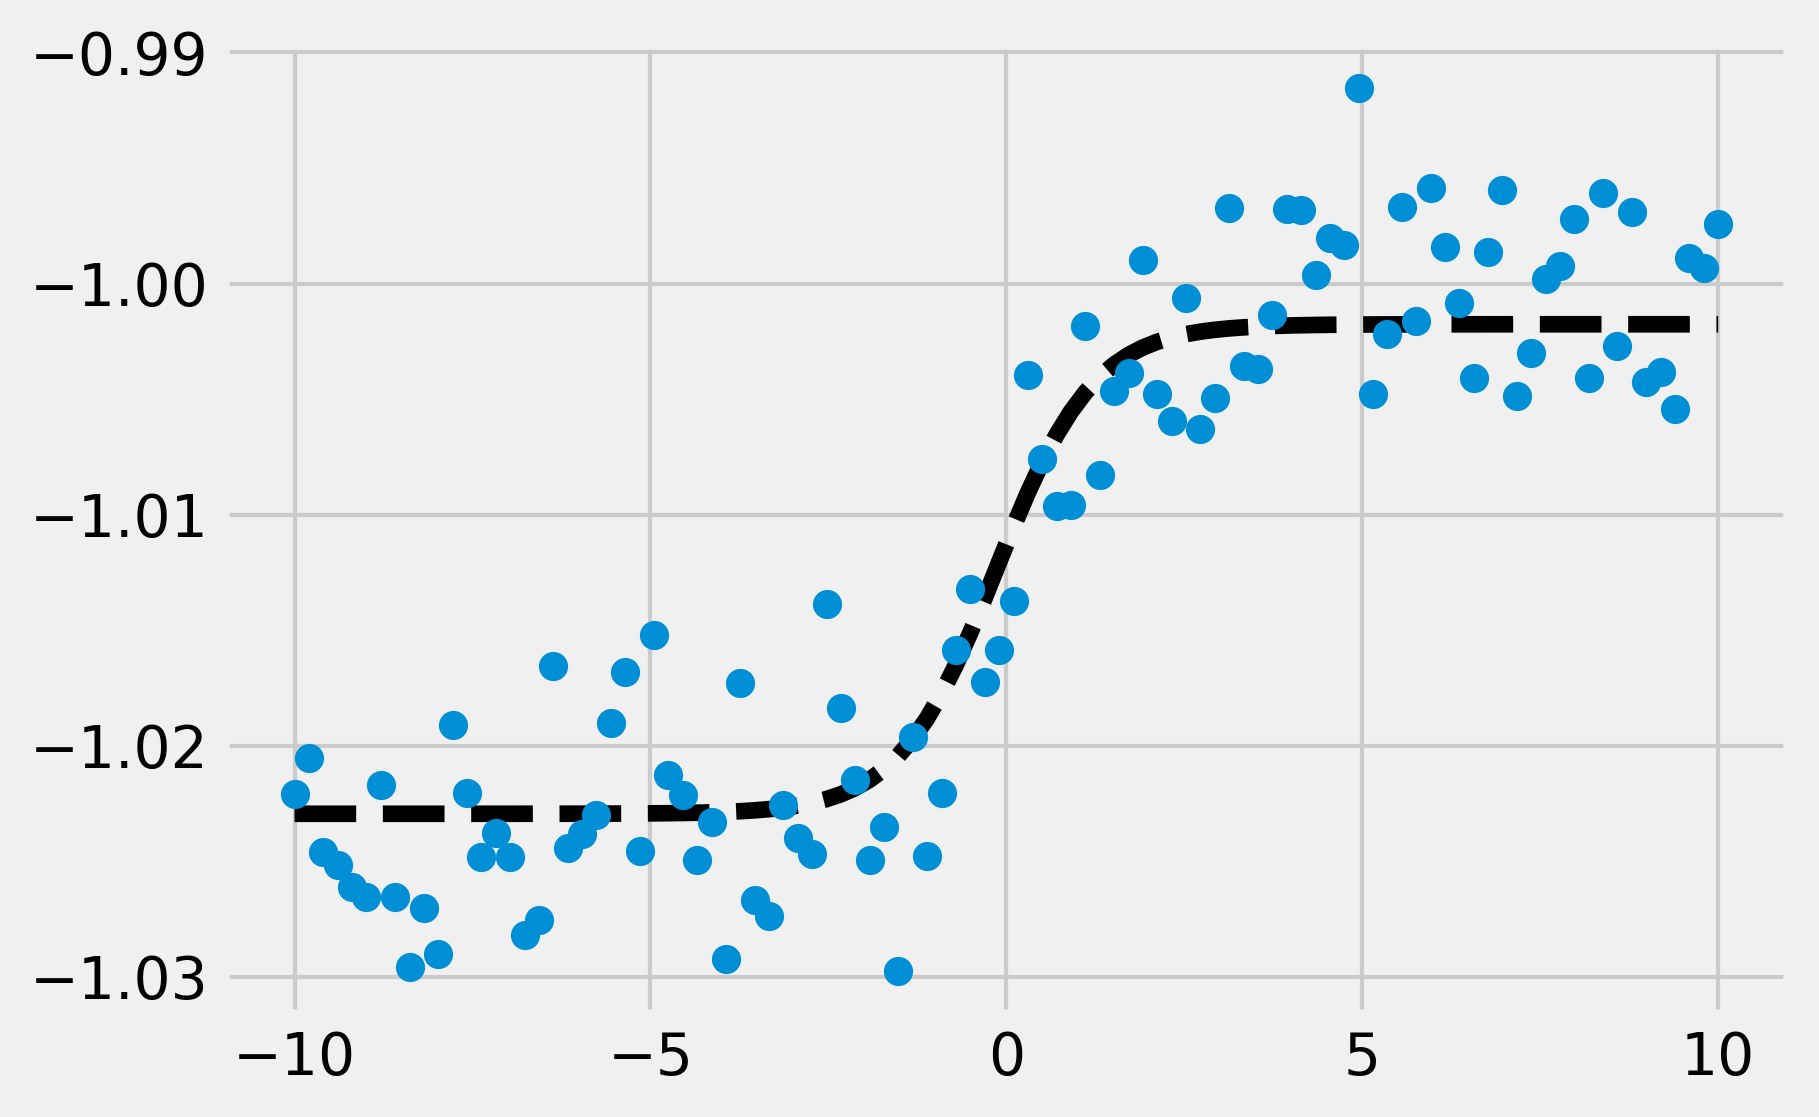
\includegraphics[width=0.55\linewidth]{figures/03_curvefitting_14_0.png}
        \caption{Example data fitting.}
    \end{figure}
\end{frame}
% \section{Recall: First-Order Optimality Conditions}

\begin{frame}{Frame Title}
    
\end{frame}
\section{Second-Order Optimality Conditions}
\subsection{}
    \begin{frame}{Motivation}
    Consider the unconstrained optimization problem of the form:
        \begin{equation}
            min\{ f(x): x \in \mathbb{R}^n\}, f: \mathbb{R}^n \longrightarrow \mathbb{R}
        \end{equation}
        $f$ non-linear.
        \begin{parchment}[Problem]
            How to find exactly minimum (or maximum) points of eq.(4)?
        \end{parchment}
    
    \end{frame}

    \begin{frame}{Definition}
        \begin{block}{Positive semidefinite matrix and positive definite matrix}
        Let $f : A^{n \times n}, d \in \mathbb{R}^n$, if :
        \begin{itemize}
            \item $\langle Ad,d \rangle \geq 0 \implies A$ is positive semidefinite $(A \succeq 0)$.
            \item $\langle Ad,d \rangle > 0, d \neq 0 \implies A$ is positive definite $(A \succ 0)$.
        \end{itemize}
        \end{block}
    \end{frame}

    \begin{frame}{Definition}
        \begin{block}{Hessian matrix and Second-order theorem}
        Let $x, \overline{x} \in \mathbb{R}^n$ and $f \in C^2$. We have:
        \begin{itemize}
            \item $Hf(x) = \bigtriangledown^2f(x) = \bigtriangledown (\bigtriangledown f(x))$ is called Hessian matrix.
            \item If $\overline{x}$ is a local minimizer $\implies \bigtriangledown f(\overline{x}) = 0, Hf(\overline{x}) \succeq 0$ (Second-order necessary condition).
            \item If $\overline{x} \in \mathbb{R}^n, \bigtriangledown f(\overline{x}) = 0, Hf(\overline{x}) \succ 0 \implies \overline{x}$ is strict local minimizer (Second-order sufficient condition ).
            \item  If $U \subseteq \mathbb{R}^n $ is a open convex set, $\overline{x} \in U, \bigtriangledown f(\overline{x}) = 0, Hf(\overline{x}) \succeq 0 \implies x$ is a global minimizer (Second-order sufficient condition for a global minimizer).
            \item  If $\bigtriangledown f(\overline{x}) = 0, Hf(x)$ is indefinite $\implies \overline{x}$ is a \textbf{saddle point} (Second-order sufficient condition for a saddle point)
        \end{itemize}
        \end{block}
    \end{frame}

    \begin{frame}{Discussion}
        \begin{block}{Proof: Second-order necessary condition for a local minimizer}
        \begin{itemize}
            \item Let $\overline{x}$ is a local minimizer, $|t|$ is small enough, $\forall d \in \mathbb{R}^n$, Then:
                \begin{equation}
                    f(\overline{x} + td) - f(\overline{x}) \geq 0
                \end{equation}
            % \item Because $t > 0$:
            %     \begin{equation}
            %         \frac{f(\overline{x} + td) - f(\overline{x})}{t} \geq 0
            %     \end{equation}
            % \item Let $t \rightarrow 0^+ \implies$eq.(3) $\geq 0; t< 0, t \rightarrow 0^- \implies$ eq.(3) $\leq 0$. Therefore $\langle \bigtriangledown f(\overline{x}), d \rangle = 0 \implies \bigtriangledown f(\overline{x}) = 0$.
            \item Because $f \in C^2$, then:
                \begin{equation}
                    f(\overline{x} +td) = f(x) + t\langle \bigtriangledown f(\overline{x}), d \rangle + \frac{t^2}{2}\langle \bigtriangledown^2 f(\overline{x})d, d \rangle + o(t^2)
                \end{equation}
            \item  We have $\langle \bigtriangledown f(\overline{x}), d \rangle = 0$. Then:
                \begin{equation}
                    0 \leq f(\overline{x} + td) - f(\overline{x}) = \frac{t^2}{2}\langle \bigtriangledown^2 f(\overline{x})d, d \rangle + o(t^2) \implies \bigtriangledown^2 f(\overline{x})d, d \rangle \geq 0 \implies \bigtriangledown^2 f(\overline{x}) \succ 0
                \end{equation}
        \end{itemize}
        \end{block}
    \end{frame}

    \begin{frame}{Discussion}
        \begin{block}{Proof: Second-order sufficient condition for a local minimizer}
        \begin{itemize}
            \item If $\bigtriangledown^2 f(\overline{x}) \succ 0$, let $\lambda $ is a smallest eigenvalue of $\bigtriangledown^2 f(\overline{x})$ $\implies \langle \bigtriangledown^2 f(\overline{x})d, d \rangle \geq \lambda ||d||^2, \forall d \in \mathbb{R}^n$.
            \item  We have $\langle \bigtriangledown f(\overline{x}), d \rangle = 0$. Then
                \begin{equation}
                f(\overline{x} + td) =  f(\overline{x}) + \frac{t^2}{2}\langle \bigtriangledown^2 f(\overline{x})d, d \rangle + o(t^2) \implies
                \frac{f(\overline{x} + td) - f(\overline{x})}{t^2} \geq \frac{\lambda ||d||^2}{2} + \frac{o(t^2)}{t^2}
                \end{equation}
            \item $|t|$ is small enough $\implies f(\overline{x} + td) - f(\overline{x}) > 0, \forall 0 \ne d \in \mathbb{R}^n\implies \overline{x}$ is strict local minimizer of $f$ in $\mathbb{R}^n$.
        \end{itemize}
        \end{block}
    \end{frame}

    \begin{frame}{Discussion}
        \begin{block}{Proof: Second-order sufficient condition for a global minimizer}
        Let $y \in U \implies \exists z \in (x, y)$:
        \begin{equation}
            f(y) = f(x) +  \langle \bigtriangledown f(x), y - x \rangle + \frac{1}{2}(y-x)^THf(z)(y-x)
        \end{equation}
        Because $\bigtriangledown f(x) > 0, Hf(x) \succeq 0 \implies f(y) \geq f(x)$. Thus, $x$ is a global minimizer of $f$ on $U$.
        \end{block}
    \end{frame}

    
    \begin{frame}{Discussion}
        \begin{block}{Consequence}
             Since: $max \{f(x)| x \in \mathbb{R}^n\} = - min\{-f(x)| x \in \mathbb{R}^n\}$, we have:
            \begin{itemize}
            \item If $\overline{x}$ is a local maximizer of $f(x) \implies \bigtriangledown f(\overline{x}) = 0 $ and $\bigtriangledown^2 f(\overline{x}) \preceq 0$  
            \item If $\bigtriangledown f(\overline{x}) = 0$ and $\bigtriangledown^2 f(\overline{x}) \prec 0$ $\implies \overline{x}$ is a strict local maximizer of $f(x)$
            \end{itemize}
        \end{block}
    \end{frame}

    \begin{frame}{Meaning of Second-Order Optimality Conditions}
    \begin{itemize}
        \item The second order condition is a filter that helps identify the nature of stationary points is a local minimum, local maximum, or saddle point. The result of the second derivative at a point $x$ tells us the slope of the tangent line.
        \item Useful in practice: Optimize for Machine Learing, Deep learing algorithmns.
    \end{itemize}
    \end{frame}

    \begin{frame}{How to find ?}
        Let $x \in A^n, f: A^n \rightarrow \mathbb{R}$:
        \begin{itemize}
            \item We differentiate once to find $\bigtriangledown f(x)$.
            \item Let $\bigtriangledown f(x) = 0$, we find all critical points.
            \item  We differentiate twice to find $\bigtriangledown ^2 f(x)$.
            \item For each point $x_0$ in step (2), calculate $\bigtriangledown ^2 f(x_0)$. If:
            \begin{itemize}
                \item $\bigtriangledown ^2 f(x_0) \succ 0 \implies x_0$ is a local minimizer (if A convex $x_0$ is a global minimizer).
                \item $\bigtriangledown ^2 f(x_0) \prec 0 \implies x_0$ is a local maximizer.
                \item $\bigtriangledown ^2 f(x_0)$ is indefinite $\implies x_0$ is a saddle points.
            \end{itemize}
        \end{itemize}
    \end{frame}

    \begin{frame}{Computational example}
        \begin{block}{Problem 1: Find all critical points of $f(x)$}
            \begin{equation}
                f(x) = x^5 - 5x
            \end{equation}
        \end{block}
        Proof: \\
        - Let $x \rightarrow +\infty \implies f(x) \rightarrow +\infty$; $x \rightarrow -\infty \implies f(x) \rightarrow -\infty$. Thus, $f(x)$ hasn't global critical points. \\
        - $f'(x) = 5x^4 -5 = 0 \Leftrightarrow x = \pm 1.$ \\
        - $f''(x) = 20x^3, f''(1) = 20 > 0, f''(-1) = -20 < 0 \implies x_1=1 $ is a local minimizer, $x_2=-1$ is a local maximizer.
    \end{frame}
    
    \begin{frame}{Computational example}
        \begin{block}{Problem 2: Find all minimizers and maximizers of $f(x, y)$}
            \begin{equation}
                f(x,y) = \frac{1}{4}(x^4 -4xy +y^4)
            \end{equation}
        \end{block}
        Proof: \\
        - We have:
        \begin{equation}
            \bigtriangledown f(x, y) = \begin{pmatrix}
                x^3 & -y \\
                -x & +y^3
            \end{pmatrix}, 
            \bigtriangledown^2 f(x, y) = \begin{pmatrix}
                3x^2 & -1 \\
                -1 & + 3y^2
            \end{pmatrix}
        \end{equation}

        - $\bigtriangledown f(x,y) = 0 \Leftrightarrow (x,y) \in \{(0,0)^T, (1,1)^T, (-1, -1)^T\}$. We have:
        \begin{equation}
            \bigtriangledown^2 f(0,0) = \begin{pmatrix}
                0 & -1 \\
                -1 & 0
            \end{pmatrix}, \bigtriangledown^2 f(1,1) =  \bigtriangledown^2 f(-1,-1) = \begin{pmatrix}
                3 & -1 \\
                -1 & 3
            \end{pmatrix}
        \end{equation}
        - Because  $\bigtriangledown^2 f(1,1) \succ 0$ and $\bigtriangledown^2 f(-1,-1) \succ 0 \implies (\pm 1, \pm 1)^T $ is strict local minimizers. $\mathbb{R}^2$ is convex set $\implies (\pm 1, \pm 1)^T$ also is global minimizers.
        
        - Because  $\bigtriangledown^2 f(0,0) \notin \{\succeq 0, \preceq 0 \} \implies (0,0)^T$ not is local critical points.
    \end{frame}

    \begin{frame}{Computational example}
        \begin{block}{Problem 3:  Consider the family of problems}
            \begin{equation}
                min f(x,y) = x^2 + y^2 +\beta xy + x + 2y
            \end{equation}
        \end{block}
        Proof: \\
        - We have:
        \begin{equation}
            \bigtriangledown f(x, y) = \begin{pmatrix}
                2x + \beta y  +1 \\
                2y + \beta x  +2
            \end{pmatrix}, 
            \bigtriangledown^2 f(x, y) = \begin{pmatrix}
                2 & \beta \\
                \beta & 2
            \end{pmatrix}
        \end{equation}

        - If $\beta \ne \pm 2 \implies$$\bigtriangledown f(x,y) = 0 \Leftrightarrow (x^*,y^*) = (2\beta -2, \beta-4) / (4-\beta^2)$.

        - If $\beta = \pm 2$, we have an inconsistent system of equations. Therefore, no critical points exist for $\beta = \pm 2$
        
       - Let $A = Hf(x,y), \lambda$ is a eigenvalue of A. We have:
       \begin{equation}
           det(A-\lambda I) = (2 - \lambda)^2 - \beta ^2 = 0 \Leftrightarrow \lambda = 2 \pm \beta
       \end{equation}

       - If $-2 < \beta < 2 \implies A \succ 0, \forall \lambda > 0 \implies (x^*, y^*)$ is global minimizers.
       
       - If $|\beta | > 2 \implies \lambda_1 \lambda_2 < 0 \implies (x^*, y^*)$ is saddle points.
    \end{frame}
\section{Important results in finite dimensions}

\subsection{Implicit function theorem}

\begin{frame}{What is implicit function?}
    If a function is written in the form of
    \begin{equation}
        y = f(x), \text{ e.g., } y = 2x^3
    \end{equation}
    is called an \textbf{explicit function}. 
    \\And sometimes functions are given in the form 
    \begin{equation}
        y - f(x) = 0 \text{ e.g., } y - 2x^3 = 0
    \end{equation}
    is called an \textbf{implicit function}.\\
    In general, \textbf{implicit function} are written in a general form as
    \begin{equation}
        F(y, x) = 0
    \end{equation}
    \footnotetext[1]{While we can always change an explicit function into an implicit function (by taking $f(x)$ to the other side of the equality) the reverse is not always true}
\end{frame}

\begin{frame}{Motivation}
    \begin{parchment}[Question]
        \begin{enumerate}
            \item Given a solution to a system of equations, are there other solutions nearby? \\=> The analytic version of the implicit function theorem.
            \item What does the set of all solutions look like near a given solution? \\=> The geometric version of the implicit function theorem.
        \end{enumerate}
    \end{parchment}
\end{frame}

\begin{frame}{Implicit function theorem}
    \begin{block}{Theorem: Implicit function theorem}
        Suppose that $U \subseteq \R^n$, and $V \subseteq \R^m$ are open sets, and $\mathbf{F}: U \times V \rightarrow \R^m$ is a function of class $C^1$. Let $(x_0, y_0) \in U \times V$ is a point such that $\mathbf{F}(x_0, y_0) = 0$ and $D_y\mathbf{F}(x_0, y_0) : \R^m \rightarrow \R^m$, the derivative of $\mathbf{F}$ w.r.t $y$, is nonsingular, i.e $D_y\mathbf{F}(x_0, y_0) \ne 0$. Then
        \begin{itemize}
            \item There exists neighborhoods $U_1 \ni x_0$ and $V_1 \ni y_0$ and a $C^1$ mapping $y: U_1 \rightarrow V_1$ such that a point $(x, y) \in U_1 \times V_1$ satisfies $\mathbf{F}(x, y) = 0$ if and only if $y = \mathbf{f}(x)$. The derivative of $y$ at $x_0$ is given by
            \begin{equation}
                D_y(x_0) = -D_y\mathbf{F}(x_0, y_0)^{-1}D_x\mathbf{F}(x_0, y_0)
            \end{equation}
            \item Moreover, if $\mathbf{F}$ is $k$-times continously differentiable, i.e., $\mathbf{F} \in C^k$, then $\mathbf{f}(x) \in C^k$.
        \end{itemize}
    \end{block}
\end{frame}

\begin{frame}{Proof of Implicit function theorem}
    At first, we need to setup something...\\
    \vspace{1cm}
    If necessary, considering the function
    \begin{equation}
        (x,y) \mapsto f(x + x_0, y+ y_0) - f(x_0, y_0)
    \end{equation}
    And, let 
    \begin{equation}
        f(x) = (f_1(x, y), \dots, f_m(x, y))
    \end{equation}
\end{frame}

\begin{frame}{Proof of Implicit function theorem}
    $Df$ is continous $\Rightarrow$ exist neighborhoods $U_0 \in \R^n$, $V_0 \in \R^m$ that
    \begin{equation}
        \begin{bmatrix}
        \nabla_yf_1(x, y_1)^{\top}\\ 
        \nabla_yf_2(x, y_2)^{\top}\\ 
        \vdots\\ 
        \nabla_yf_m(x, y_m)^{\top}
        \end{bmatrix}
    \end{equation}
    is invertible for all $(x, y_i) \in U_0 \times V_0$.
\end{frame}

\begin{frame}{Proof of Implicit function theorem}
    \textbf{Question}: Is every $x \in U_0$, then there exists at most one $y \in V_0$ such that $f(x, y) = 0$.
    \vspace{0.5cm}
    By contradiction, suppose that $\exists y, z \in V_0, y \ne z, f(x,y) = f(x,z) = 0$. Due the mean value theorem, $\exists y_i \in (y, z)$ that
    \begin{equation}
        f_i(x,z) - f_i(x,y) = \left \langle \nabla_yf_i(x,y_i), z -y \right \rangle
    \end{equation}
    And the previous matrix is non-singular, so $y = z$.
\end{frame}

\begin{frame}{Proof of Implicit function theorem}
    Let $\overline{B}_r(0) \subseteq V_0$
    \begin{itemize}
        \item $f(0, y) \ne 0, \forall y \in S_r(0) := \{y \in \R^l : \left \| y \right \| = r\}$ due to $f(0,0) = 0$.
        \item $\exists \alpha > 0, \left \| f(0, y) \geq \alpha \right \|, \forall y \in S_r(0)$ due to $f$ is continous.
    \end{itemize}
\end{frame}

\begin{frame}{Proof of Implicit function theorem}
    Consider the function 
    \begin{equation}
        F(x, y) := \left \| f(x, y) \right \|^2 = \sum_{i=1}^mf_i(x, y)^2
    \end{equation}
    that satisfies the properties 
    \begin{itemize}
        \item $F(0, y) \geq \alpha > 0, \forall y \in S_r(0)$
        \item $F(0, 0) = 0$
    \end{itemize}
\end{frame}

\begin{frame}{Proof of Implicit function theorem}
    Because $F$ is continous function, $\exists U_1 \subseteq U_0$ of $0 \in \R^n$ such that
    \begin{equation}
        F(x,y) \geq \frac{\alpha}{2}, F(x, 0) \leq \frac{\alpha}{2} \forall x \in U_1, y \in S_r(0)
    \end{equation}
    fixed $x \in U_1$, function $y \mapsto F(x, y)$ achieves its minimum on $\overline{B}_r(0)$ at $y(x)$ in the interior of $\overline{B}_r(0)$
    \begin{equation}
        D_yF(x,y(x)) = 2D_yf(x, y(x))f(x,y(x)) = 0
    \end{equation}
    And the matrix $D_yf(x, y(x))$ is non-singular, so that
    \begin{equation}
        f(x,y(x)) = 0
    \end{equation}
\end{frame}

\begin{frame}{Proof of Implicit function theorem}
    Writting $\Delta y := y(x+\Delta x) - y(y)$, by the mean value theorem
    \begin{equation}
        0 = D_xf(\widetilde{x}, \widetilde{y})\Delta x + D_yf(\widetilde{x}, \widetilde{y})\Delta y
    \end{equation}
    for some point $(\widetilde{x}, \widetilde{y})$ one the line segment between $(x, y(x))$ and $(x + \Delta x, y(x + \Delta x))$. And as $\left \| \Delta x \right \| \rightarrow 0$,  $\left \| \Delta y \right \| \rightarrow 0$, thus lead $y(x)$ is continous.
    \vspace{1cm}
    And by Taylors formula and continuity of $y(x)$, we prove that $y(x)$ is Fréchet differentiable.
    \vspace{1cm}
    If $f \in C^2$, then $y(x) \in C^2$. And in general, if $C^k$, we prove by induction on $k$ that $y(x)$ is $C^k$.
\end{frame}

\begin{frame}{Discussion about the analytic meaning}
    \begin{parchment}[Problem]
        Solving the equation below:
        \begin{equation}
            f(x, y) = 0
        \end{equation}
        for $y$ as a function of $x$, and say $y = f(x)$
    \end{parchment}
    If we have a solution $b = f(a)$, then in principle it is possible to solve for $x$ near $a$, if the crucial hypothesis $D_yf(a, b) \ne 0$ holds.\\
    In this meaning, Implicit function theorem is a theorem about the \textbf{possibility of solving a system of nonlinear equations}.
\end{frame}

\begin{frame}{Discussion about the geometric meaning}
    There are 3 natural ways to represent a curve $S \subseteq \R^n$
    \begin{itemize}
        \item As a graph
        \item As a level set
        \item Parametrically
    \end{itemize}
\end{frame}

\begin{frame}{Discussion about the geometric meaning}
    Considering the case $n = 2$
    \begin{itemize}
        \item Graph: \begin{equation}
        \left. 
        \begin{array}{c}
        S = \{ (x,y) \in \R^2:  \ y = f(x) \text{ for }x\in I\}\\
        \text{OR} \\
        S = \{ (x,y) \in \R^2:  \ x = f(y) \text{ for }y\in I\}
        \end{array}\right\}
        \label{graph}
        \end{equation}
        for some $f:I\to \R$, where $I\subseteq \R$ is an interval.
        \item Level set, is, a set of the form
        \begin{equation}
            S    = \{ (x,y)\in U : F(x,y) = c \} 
        \label{locus}\end{equation}
        for some open $U\subseteq \R^2$, some $F:U\to \R$, some $c\in \R$.
        \item Parametrically, in the form
        \begin{equation}
        S    = \{  \mathbf f(t) :  \ t\in I \} 
        \label{parametrically}\end{equation}
        for some interval $I\subseteq \R$, and some $\mathbf f:I\to \R^2$
    \end{itemize}
\end{frame}

\begin{frame}{Discussion about the geometric meaning}
    \begin{figure}[h!]
        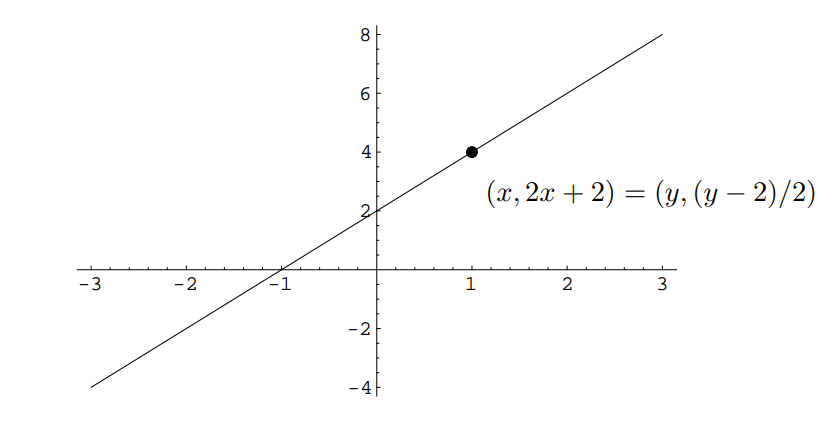
\includegraphics[width=0.75\linewidth]{figures/implicit_function_example01.png}
        \caption{The line $2x − y + 2 = 0$ as the graph of $f(x) = 2x + 2$ or of $g(y) = (y − 2)/2$}
    \end{figure}
\end{frame}

\begin{frame}{Discussion about the geometric meaning}
    \begin{figure}[h!]
        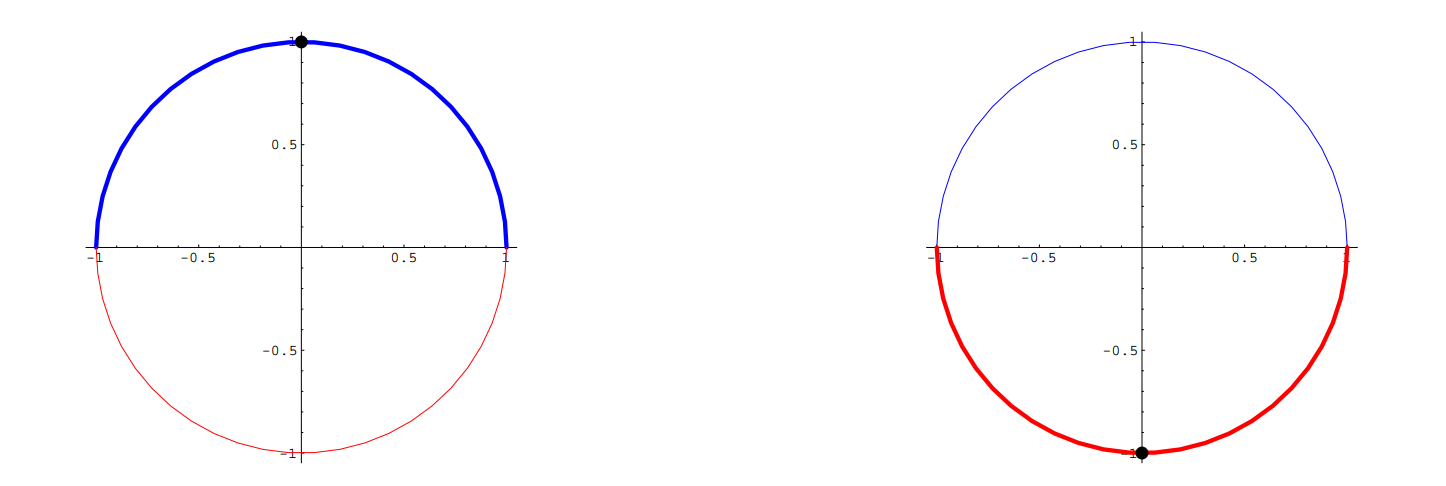
\includegraphics[width=0.75\linewidth]{figures/implicit_function_example02.png}
        \caption{The thick arcs are the graphs of $x \mapsto \pm \sqrt{1-x^2}$}
    \end{figure}
\end{frame}

\begin{frame}{Discussion about the geometric meaning}
    \begin{figure}[h!]
        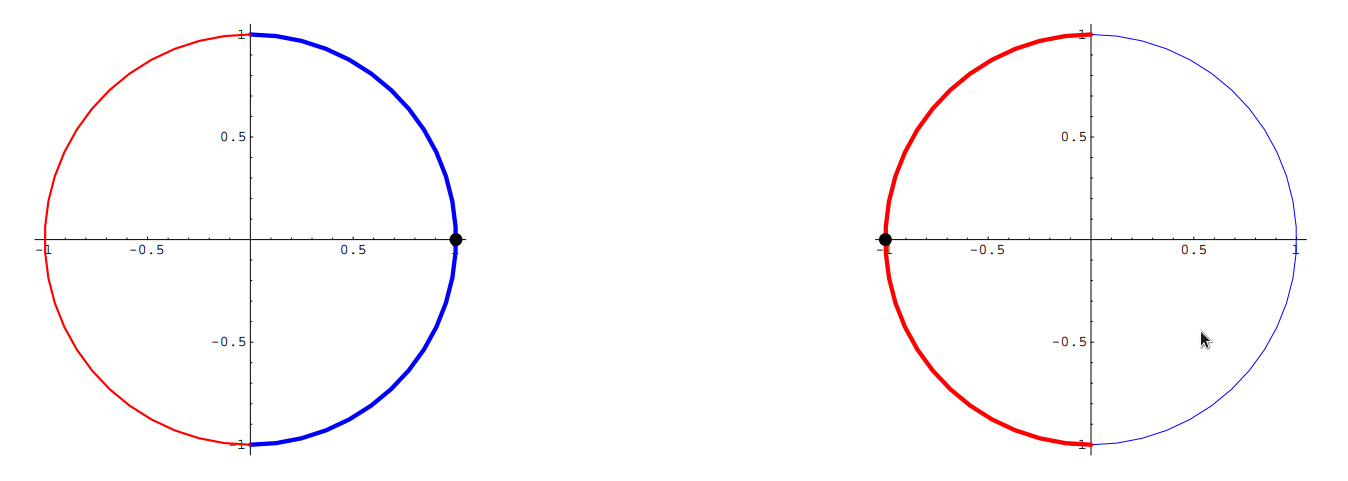
\includegraphics[width=0.75\linewidth]{figures/implicit_function_example03.png}
        \caption{The thick arcs are the graphs of $y \mapsto \pm \sqrt{1-y^2}$}
    \end{figure}
\end{frame}

\begin{frame}{Discussion about the geometric meaning}
    \begin{figure}[h!]
        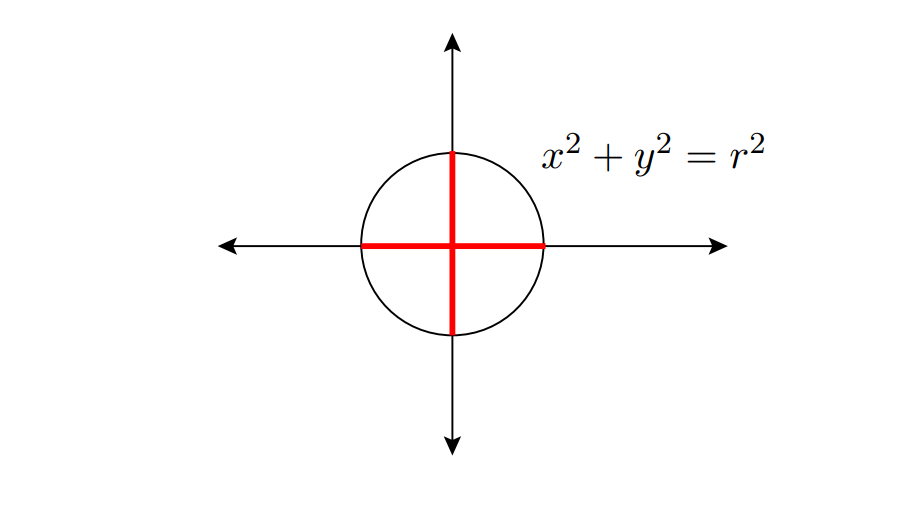
\includegraphics[width=0.75\linewidth]{figures/implicit_function_example04.png}
        \caption{Can the thick line segments be a graph?}
    \end{figure}
\end{frame}


\begin{frame}{Why the Implicit Function Theorem is a great theorem?}
    \begin{parchment}[Fact]
        With given $k$ \text{nonlinear equations} in $k$ unknowns:
        \begin{itemize}
            \item It is \textbf{impossible to solve}.
            \item It is often \textbf{impossible to determine whether it has any solutions}.
        \end{itemize}
    \end{parchment}
    The Implicit Function Theorem allows us to (partly) reduce impossible questions about systems of nonlinear equations to straightforward questions about systems of linear equations. 
\end{frame}

% \begin{frame}{Limitation of the Implicit Function Theorem}
%     Some limitation of the Implicit Function Theorem
%     \begin{itemize}
%         \item 
%     \end{itemize}
% \end{frame}

\begin{frame}{Some special cases of the implicit function theorem}
    \begin{block}{Theorem: Implicit function theorem, $m=n=1$}
        Suppose that $F$ is real-valued $C^1$ function defined for all $(x, y)$ in open set $U\times V \subseteq \R^2$.
        \begin{itemize}
            \item If $f(a, b) = 0$ and $\partial_yf(a, b) \ne 0$, then the equation
            \begin{equation}
                F(x, y) = 0
            \end{equation}
            implicitly determines $y$ as a $C^1$ function of $x$, i.e., $y = f(x)$, for $x$ near $a$.  Moreover $f(a) = b$.
            \item If $f(a, b) = 0$ and $\partial_xf(a, b) \ne 0$, then the equation
            \begin{equation}
                F(x, y) = 0
            \end{equation}
            implicitly determines $x$ as a $C^1$ function of x, i.e., $x = f(y)$, for $y$ near $b$.  Moreover $f(b) = a$.
        \end{itemize}
    \end{block}
\end{frame}

\begin{frame}{Some special cases of the implicit function theorem}
    \begin{block}{Theorem: Implicit function theorem, $n=2, m=1$}
    Suppose that $F$ is a scalar function of class $C^1$ function defined for all $(x, y, z)$ in open set $U\times V \subseteq \R^3$.
    \begin{itemize}
        \item If $f(a, b, c) = 0$ and $\partial_zf(a, b, c) \ne 0$, then the equation
            \begin{equation}
                F(x, y, x) = 0
            \end{equation}
            implicitly determines $z$ as a $C^1$ function of $(x, z)$, i.e., $z = f(x, y)$ for $(x, y)$ near $(a, b)$. Moreover, $f(a, b) = c$.
        \item Similarly, we also have results in the cases: $f(a, b, c) = 0$ and $\partial_yf(a, b, c) \ne 0$; and $f(a, b, c) = 0$ and $\partial_xf(a, b, c) \ne 0$
    \end{itemize}
    \end{block}
\end{frame}

\begin{frame}{Some special cases of the implicit function theorem}
    \begin{block}{Theorem: Implicit function theorem, $n=1, m=2$}
    Suppose that $\mathbf{F} = (F_1, F_2)$ is function $U \times V \rightarrow \R^2$ of class $C^1$ defined for all $(x, y, z)$ in open set $U\times V \subseteq \R^3$.
    \begin{itemize}
        \item If $\mathbf{F}(a, b, c) = \mathbf{0}$ and 
        \begin{equation}
            \begin{vmatrix}
             \partial_yF_1 & \partial_zF_1\\ 
             \partial_yF_2 & \partial_zF_2
            \end{vmatrix} \ne 0
        \end{equation} 
        then
        \begin{equation}
            \mathbf{F}(x, y, z) = \mathbf{0} \Leftrightarrow \begin{cases}
                F_1(x, y, z) = 0\\
                F_2(x, y, z) = 0\\
            \end{cases}
        \end{equation}
        implicitly determines $(y, z)$ as a $C^1$ function of $x$, i.e., $(y, z) = \mathbf{f}(x)$, for $x$ near $a$. Moreover, $\mathbf{f}(b, c) = f(a)$.
        \item Similarly, we also have results in the remain cases.
    \end{itemize}
    \end{block}
\end{frame}

\begin{frame}{Computational example 1}
    % \begin{parchment}[Problem 01]
    %     Considering the general $F: \R^3 \rightarrow \R$ of class $C^1$. Suppose that at a point $(a,b,c)\in \R^3$, we have $F(a,b,c) = 0, \partial_z F(a,b,c)\ne 0$. Does the equation implicitly determine $z$ as a function $f(x, y)$ for $(x,y)$ near $(a, b)$ with $f(a, b) = c$? If so, find a formula for $\partial_x f(x,y)$, and evaluate it at $(x, y) = (a, b)$.
    % \end{parchment}
    \begin{parchment}[Problem 01]
        Consider the equation
        \begin{equation}
            F(x,y,z) = xy+ xz \ln(yz)  =1
        \end{equation}
        We know that $(1, 1, 1)$ is a solution. Does the equation implicitly determine $z$ as a function $f(x, y)$ for $(x,y)$ near $(1, 1)$ with $f(1, 1) = 1$? If so, find a formula for $\partial_x f(1, 1)$, and evaluate it at $(1, 1) = (1, 1)$.
    \end{parchment}
\end{frame}

\begin{frame}{Computational example 1}
    We have
    \begin{equation}
        \partial_zF = xln(yz) + x
    \end{equation}
    And at $(x, y, z) = (1, 1, 1)$, $F(1, 1, 1) = 1$. So the Implicit Function Theorem guarantees that there is a function $f(x, y)$, defined for $(x, y)$ near $(1, 1)$ such that
    \begin{equation}
        F(x, y,z) = 1 \text{ when } z = f(x, y)
    \end{equation}
    To find $\partial_xf$, by using the original equation that defines $z$ as a function of $(x, y)$ to differentiate both sides with respect to $x$.
    \begin{equation}
        y + zln(yz) + x\dfrac{\partial z}{\partial x}ln(yz) + \dfrac{xz}{yz}y\dfrac{\partial z}{\partial x} = 0 \Leftrightarrow \dfrac{\partial z}{\partial x} = - \dfrac{y + zln(yz)}{x + xln(yz)}
    \end{equation}
    Evaluating at $(x, y, z) = (1, 1, 1)$, and solving for $\dfrac{\partial z}{\partial x}$. We have:
    \begin{equation}
        1 + \dfrac{\partial z}{\partial x} = 0 \Leftrightarrow \dfrac{\partial z}{\partial x} = -1
    \end{equation}
\end{frame}

\begin{frame}{Computational example 2}
    \begin{parchment}[Problem 02]
        Consider the system of equations
        \begin{align}
            F_1(x,y,u,v) = xye^u +  \sin(v-u) &= 0\\\
            F_2(x,y,u,v)  =(x+1)(y+2)(u+3)(v+4) - 24 &=0
        \end{align}
        We know that $(0, 0, 0, 0)$ is a solution. Does the system of equations implicitly determine $(u, v$ as a function of $(x, y)$, i.e., $(u,v) = \mathbf{f}(x, y)$ for $(x, y)$ near $(0, 0)$? If so, find a formula for $\partial_x \mathbf{f}(x, y)$ at $(x, y) = (0, 0)$ 
    \end{parchment}
\end{frame}

\begin{frame}{Computational example 2}
    Let $\mathbf F = \binom{F_1}{F_2}$. Then
    \begin{equation}
        \left(\begin{array}{ll}
        \partial_u F_1&\partial_v F_1\\\
        \partial_u F_2&\partial_v F_2
        \end{array}
        \right)  \ = \ 
        \left(\begin{array}{cc}
        xye^u  - \cos(v-u)&\cos(v-u)\\\
        (x+1)(y+2)(v+4)&(x+1)(y+2)(u+3)
        \end{array}
        \right)
    \end{equation}
    At $(x,y,u,v) = (0,0,0,0)$,
    \begin{equation}
        \left(\begin{array}{ll}
        \partial_u F_1(0,0,0,0)&\partial_v F_1(0,0,0,0)\\\
        \partial_u F_2(0,0,0,0)&\partial_v F_2(0,0,0,0)
        \end{array}\right)
        = \left(\begin{array}{rr}
        -1&1\\ 8&6
        \end{array}
        \right)
    \end{equation}
    This matrix is invertible, so the theorem guarantees that the equations implicitly determine $(u, v)$ as a function of $(x, y)$
\end{frame}

\begin{frame}{Computational example 2}
    Find $\partial_x \mathbf f = \binom{\partial_x f_1}{\partial_x f_2}$, where $\binom uv = \mathbf f(x,y) = \binom{f_1(x,y)}{f_2(x,y)}$. Considering equations below:
    \begin{align}
        \begin{aligned}
            xye^u +  \sin(v-u) &= 0\\\
            (x+1)(y+2)(u+3)(v+4) - 24 &=0.
        \end{aligned}
    \end{align}
    and differentiate everything with respect to $x$:
    \begin{align}
        \begin{aligned}
            ye^u + \left( xy e^u - \cos(v-u)\right) \frac{\partial u}{\partial x} + \cos(v-u)\frac{\partial v}{\partial x} &= 0\\\
            (y+2)(u+3)(v+4) +(x+1)(y+2)(v+4)\frac{\partial u}{\partial x} +(x+1)(y+2)(u+3)\frac{\partial v}{\partial x}   &=0.
        \end{aligned}
    \end{align}
\end{frame}

\begin{frame}{Computational example 2}
    At $(x,y,u,v) = (0,0,0,0)$,
    \begin{align}
    \left(\begin{array}{rr}
    -1&1\\\ 8&6
    \end{array}
    \right)\binom
    {\frac{\partial u}{\partial x}}
    {\frac{\partial v}{\partial x}} = \binom 0{-24}.
    \label{concrete}\end{align}
    And
    \begin{equation}
            \binom{\frac{\partial u}{\partial x}}
{\frac{\partial v}{\partial x}} = \frac{1}{-14}
\left(
\begin{array}{rr}
6&-1 \\\
-8&-1
\end{array}
\right)\binom0 {-24} =  -\binom{12/7}{12/7}.
    \end{equation}
\end{frame}

\subsection{Inverse function theorem}

\begin{frame}{What is Transformations?}
    \begin{parchment}{Fact}
        Let $U$, and $V$ be two open subsets of $\R^n$. Considering functions as
        \begin{equation}
            \mathbf{f}: U \rightarrow V
        \end{equation}
        is called \emph{transformation}. \\
        If $\mathbf{f}$ is a bijection (that is, both one-to-one and onto). Then implies that $\mathbf{f}^{-1}: V \rightarrow U$ exists. And both $\mathbf{f}$, $\mathbf{f}^{-1}$ are class of $C^1$.
    \end{parchment}
    
\end{frame}

\begin{frame}{Example}
    Considering the transformation of Cartesian grid by using the linear mapping $\mathbf f(x,y) = (2y-x,x+y)$.
    \begin{columns}
        \begin{column}{0.5\textwidth}
            \begin{figure}[h!]
                
\includegraphics[width=0.95\linewidth]{figures/Grid.jpg}
                \caption{Before transformation.}
                \label{fig:example-astatic-knowledge-graph}
            \end{figure}
        \end{column}
        \begin{column}{0.5\textwidth}  %%<--- here
            \begin{figure}[h!]
                
\includegraphics[width=0.95\linewidth]{figures/linear_after.jpg}
                \caption{After transformation.}
                \label{fig:example-astatic-knowledge-graph}
            \end{figure}
        \end{column}
    \end{columns}
\end{frame}

\begin{frame}{The Inverse Function Theorem}
    \begin{block}{Theorem: The Inverse Function Theorem}
        Let $\mathbf{f}$ be a $C^1$ map from a neighborhood of $x_0 \in \R^n$ into $\R^n$. If $D\mathbf{f}(x_0)$ is non-singular, then there exist neighborhoods $U \ni x_0$ and $V \ni y_0 = \mathbf{f}(x_0)$ such that $ \mathbf{f} : U \rightarrow V$ is a $C^1$ diffeomorphism\footnotemark, and 
        \begin{equation}
            D\mathbf{f}^{-1}(y) = D\mathbf{f}(x)^{-1} \text{ for all} (x, y) \in U \times V, y = \mathbf{f}(x)
        \end{equation}
        Moreover, if $\mathbf{f}$ is $C^k$, then $\mathbf{f}$ is a $C^k$ diffeomorphism on $U$.
    \end{block}
    \footnotetext{A diffeomorphism is an isomorphism of smooth manifolds. It is an invertible function that maps one differentiable manifold to another such that both the function and its inverse are continuously differentiable.}
\end{frame}

\begin{frame}{Proof of The Inverse Function Theorem}
    We can define the function 
    \begin{equation}
        F(x, y) = f(x) - y
    \end{equation}
    and, find that
    \begin{equation}
        D_xF(x_0, y) = Df(x_0)
    \end{equation}
    is non-singular.
    \vspace{1cm}
    And apply the Implicit function theorem to $F$.
\end{frame}

\begin{frame}{The usage of Implicit Function Theorem}
    \begin{parchment}{Problem}
        Suppose that given $\mathbf{f}: U \rightarrow V$, and $\mathbf{y}  \in V$, find $\mathbf{x}$ by solving 
        \begin{equation}
            \mathbf{f}(\mathbf{x}) = \mathbf{y}
        \end{equation}
    \end{parchment}
    \begin{parchment}{Fact}
        This problem is often an impossible problem to solve handle.
    \end{parchment}
    
\end{frame}
\begin{frame}{The usage of Implicit Function Theorem}
    \begin{parchment}[The Inverse Function Theorem says]
        If we know that $\mathbf{f}(\mathbf{a}) = \mathbf{b}$, then for $\mathbf{y}$ near $\mathbf{b}$, the solvability of the \textbf{nonlinear system} can be established by considering a \textbf{much easier} question about linear algebra, whether the matrix $D\mathbf{f}(a)$ is invertible.
    \end{parchment}
\end{frame}

\begin{frame}{Computational example}
    \begin{parchment}[Problem 03]
       Determine whether the system
        \begin{equation}
            \begin{cases}
                u(x, y, z) = x + xyz\\
                v(x, y, z) = y + xy\\
                w(x, y, z) = z + 2x + 3z^2
            \end{cases}
        \end{equation}
        can be solved for $x, y, z$ in terms of $u, v, w$ near $p = (0, 0, 0)$.
    \end{parchment}
\end{frame}

\begin{frame}{Computational example}
    Let $\mathbf{F}(x, y,z) = (u, v, w)$, then
    \begin{equation}
        D\mathbf{F}(p) = \begin{pmatrix}
         u_x& u_y & u_z\\ 
         v_x& v_y & v_z\\ 
         w_x& w_y & w_z
        \end{pmatrix}(p)
        = \begin{pmatrix}
         1+yz& xz & xy\\ 
         y& 1+x & 0\\ 
         2& 0 & 1+6z
        \end{pmatrix}(p)
        = \begin{pmatrix}
         1& 0 & 0\\ 
         0& 1 & 0\\ 
         2& 0 & 1
        \end{pmatrix}
    \end{equation}
    Due to,
    \begin{equation}
        \begin{vmatrix}
         1& 0 & 0\\ 
         0& 1 & 0\\ 
         2& 0 & 1
        \end{vmatrix} = 1 \ne 0
    \end{equation}
    By the Inverse Function Theorem, the inverse function $F^{-1}(u,v,w)$ exists near $p=(0, 0,0)$, i.e., we can solved for $x, y, z$ in terms of $u, v, w$ near $p = (0, 0, 0)$.
\end{frame}

\subsection{Lyusternik theorem}

\begin{frame}{The Lyusternik theorem}
    \begin{block}{Definition of tangent direction}
        Let $M$ be a non-empty subset of $\R^n$ and $x \in M$. A vector $d \in R^n$ is called a tangent direction of $M$ at $x$ if there exist a sequence $x_n \in M$ converging to $x$ and a non-negative seqence $\alpha_n$ such that
        \begin{equation}
            \underset{n\rightarrow\infty}{\lim}\alpha_n(x_n-x)=d
        \end{equation}
        The tangent cone of $M$ at $x$, donated by $T_M(x)$, is the set of all tangent direction of $M$ at $x$.
    \end{block}
\end{frame}

\begin{frame}{The Lyusternik theorem}
    \begin{block}{Theorem: The Lyusternik theorem}
        Let $\mathbf{F}: U \rightarrow \R^m$ be $C^1$ map, where $U \subset \R^n$ be an open set. Let $M = \mathbf{F}^{-1}(\mathbf{F}(x_0))$ be the level set of a point $x_0 \in U$. If the derivative $D\mathbf{F}(x_0)$ is a linear map onto $\R^m$, then the tangent cone of $M$ is the null space of the linear map $D\mathbf{F}(x_0)$, that is,
        \begin{equation}
            T_M(x_0) = \{d \in \R^n: D\mathbf{F}(x_0)d=0\}
        \end{equation}
    \end{block}
\end{frame}

\begin{frame}{The proof of Lyusternik theorem}
    If nescessary, we will consider the function
    \begin{equation}
        x \mapsto f(x + x_0) - f(x_0)
    \end{equation}
    Assume that $x_0 = 0$, and $f(x_0) = 0$. And, define $A:= Df(0)$
\end{frame}

\begin{frame}{The proof of Lyusternik theorem}
    Now, we will prove that
    \begin{equation}
        T_M(0) \subseteq \text{Ker}A
    \end{equation}
    If $d \in T_M(0)$, then there exists points $x(t) = td + o(t) \in M$. We have:
    \begin{align}
        \begin{aligned}
            f(x) &=0\\
            f(x(t)) & = 0\\
            f(td + o(t) + 0) &= 0\\
            tDf(0)(d) + o(t) + f(0) &= 0\\
            Df(0)(d) + \frac{o(t)}{t} &= 0\\
            \lim_{t \rightarrow \infty}\left(Df(0)(d) + \frac{o(t)}{t}\right) &= 0\\
            Df(0)(d) &= 0
        \end{aligned}
    \end{align}
\end{frame}

\begin{frame}{The proof of Lyusternik theorem}
    Idea to prove the reverse inclusion: the equation $f(x) = 0$ can be written as $f(y,z) = 0$in a form that is suitable for applying the implicit function theorem.
\end{frame}

\begin{frame}{The proof of Lyusternik theorem}
    Define $K:= \text{Ker}A$, and $L := K^{\perp}$. Since $A:= Df(0)$ is onto $\R^m$, we can identify $K$ and $L$ with $\R6{n-m}$ and $\R^m$ respectively, by introducing a suitable basis in $\R^n$.\\
    For a point $x \in \R^n$ in form that $x = (y, z) \in K \times L$, we have $A = [D_yf(0), D_zf(0)]$, and
    \begin{equation}
        0 = A(K) = \{A(d_1, 0) : d_1 \in R^{n-m} = D_yf(0)(\R^{n-m}\}
    \end{equation}
    so that $D_yf(0) = 0$. And due to $A$ has rank $m$, so that $D_zf(0)$ is non-singular.
\end{frame}

\begin{frame}{The proof of Lyusternik theorem}
    Following the Implicit function theorem, there exists neighborhoods $U_1 \subseteq \R^m$, and $U_2 \subseteq \R^{n-m}$ around the origin and a $C^1$ map $\alpha: U_1 \rightarrow U_2, \alpha(0) = 0$, such that $x = (y, z) \in U_1 \times U_2$ satisfies $f(x) = 0$ if and only if $z = \alpha(y)$. The equation $f(x) = 0$ can be written as $f(y, \alpha(y))$. Differentiating this equation
    \begin{align}
        \begin{aligned}
            D_yf(y, \alpha(y)) + D_zf(y, \alpha(y)D_\alpha(y) = 0
        \end{aligned}
    \end{align}
    At $x = 0$, $D_yf(0) = 0$, and $D_zf(0)$ is non-singular, so that $D_\alpha(0) = 0$
\end{frame}

\begin{frame}{The proof of Lyusternik theorem}
    If $|y|$ is small:
    \begin{equation}
        \alpha(y) = \alpha(0) + D\alpha(0)y + o(y) = o(y)
    \end{equation}
    Let $d = (d_1, 0) \in K$, as $t \rightarrow 0$, the point $x(t) := (td_1, \alpha(td_1)) = (td_1, o(t))$ lies in $M$. And that is $f(x(t)) = 0$, and satisfies 
    \begin{equation}
        \frac{x(t) - td}{t} = \frac{(0, o(t))}{t} \rightarrow 0
    \end{equation}
    This implies that $K \subseteq T_M(0)$.
\end{frame}

\begin{frame}{The usage of the Lyusternik theorem}
    The usage of the Lyusternik theorem (finite version)
    \begin{itemize}
        \item Application in multi-objective optimization \cite{jimenez2002finite}
    \end{itemize}
\end{frame}
\section{Conclusion}

\begin{frame}{Conclusion \& Future working}
    Conclusion
    \begin{itemize}
        \item Fully presentation about second conditional optimality
        \item Fully presentation about implicit function theorem, inverse function theorem, and Lyusternik theorem.
    \end{itemize}
    Future work
    \begin{itemize}
        \item Give more detail about the proof of these theories and theorems.
        \item Give more examples and applications of these theories and theorems.
    \end{itemize}
\end{frame}

% normal frame
% \section{Bayesian Statistics Tutorial}
% \subsection{}
% \begin{frame}
%     \frametitle{Basics}
%     conditional probabilities:
%     $$
%     p(x|y) \coloneqq \frac{p(x,y)}{p(y)}
%     $$
%     the joint probalility of $x$ and $y$:
%     $$
%     p(x,y)=p(x|y)p(y)=p(y|x)p(x)
%     $$

%     \begin{block}{Theorem: Bayes Rule}
%     Denote by X and Y random variables then the following holds
%     $$
%     p(y|x)=\frac{p(x|y)p(y)}{p(x)}
%     $$
%     \end{block}

% \end{frame}

% \begin{frame}
%     \frametitle{An Example}

%     \begin{parchment}[Question]
%         Assume that a patient would like to have such a test carried out on him. The physician recommends a test which is guaranteed to detect HIV-positive whenever a patient is infected. On the other hand, for healthy patients it has a $1\%$ error rate. That is, with probability 0.01 it diagnoses a patient as HIV-positive even when he is, HIV-negative. \uwave{Moreover, assume that $0.15\%$ of the population is infected.}
%         \\[1ex]
%         Now the patient has the test carried out and the test returns HIV-negative. In this case, logic implies that he is healthy, since the test has $100\%$ detection rate. In the converse case things are not quite as straightforward.
%         \\[1ex]
%         So what's the $p(X = \mathtt{HIV+}|T = \mathtt{HIV+})$?
%     \end{parchment}
    
% \end{frame}

% \begin{frame}
%     \frametitle{An Example}

%     \center{
%     \begin{tabular}{ c | c c }
%         $p(t|x)$ & $X = \mathtt{HIV-}$ & $X=\mathtt{HIV+}$ \\
%         \hline
%         $T=\mathtt{HIV-}$ & 0.99 & 0 \\
%         $T=\mathtt{HIV+}$ & 0.01 & 1
%     \end{tabular}
%     }

%     $$
%     p(X = \mathtt{HIV+}) = 0.0015
%     $$
% \end{frame}

% \begin{frame}
%     \frametitle{An Example}

%     By Bayes rule we may write
%     $$
%     p(X = \mathtt{HIV+}|T=\mathtt{HIV+}) = \frac{p(T=\mathtt{HIV+}|X=\mathtt{HIV+})p(X=\mathtt{HIV+})}{p(T=\mathtt{HIV+})}
%     $$

%     While we know all terms in the numerator, $p(T = \mathtt{HIV+})$itself is unknown. That said, it can be computed via
%     \begin{align}
%     \nonumber p(T=\mathtt{HIV+}) &= \sum_{x \in \{\mathtt{HIV+}, \mathtt{HIV-}\}}p(T=\mathtt{HIV+},x) \\
%     \nonumber &= \sum_{x \in \{\mathtt{HIV+}, \mathtt{HIV-}\}}p(T=\mathtt{HIV+}|x)p(x) \\
%     \nonumber &= 1.0 \cdot 0.0015 + 0.01 \cdot 0.9985
%     \end{align}

%     Substituting back into the conditional expression yields
%     $$
%     p(X = \mathtt{HIV+}|T=\mathtt{HIV+}) = \frac{1.0 \cdot 0.0015}{1.0 \cdot 0.0015 + 0.01 \cdot 0.9985} = 0.1306
%     $$

% \end{frame}


% \begin{frame}
%     \frametitle{How can we improve the diagnosis}

%     % Define block styles
%     \tikzset{
%         grayCircle/.style = {
%             draw,
%             circle,
%             node distance=2.5cm,
%             minimum size=1.5cm,
%             fill=black!20
%         }
%     }

%     \center
%     \begin{tikzpicture}
%         \node[grayCircle] (age) {age};
%         \node[grayCircle, right of=age, style={fill=none}] (x) {x};
%         \node[grayCircle, right of=x, yshift=1.25cm] (t1) {test 1};
%         \node[grayCircle, below of=t1] (t2) {test 2};
%         \draw[->, >=latex] (age) -- (x);
%         \draw[->, >=latex] (x) -- (t1);
%         \draw[->, >=latex] (x) -- (t2);
%     \end{tikzpicture}

%     \begin{figure}
%         \caption{A graphical description of our HIV testing scenario. Knowing the age of the patient influences our prior on whether the patient is HIV positive (the random variable X). The outcomes of the tests 1 and 2 are independent of each other given the status X. We observe the shaded random variables (age, test 1, test 2) and would like to infer the un-shaded random variable X.}
%     \end{figure}

% \end{frame}


% \begin{frame}
%     \frametitle{How can we improve the diagnosis}

%     \begin{parchment}[Including additional observed random variables]
%     One way is to obtain further information about the patient and to use this in the diagnosis. For instance, information about his age is quite useful. Suppose the patient is 35 years old. In this case we would want to compute $p(X = \mathtt{HIV+}|T = \mathtt{HIV+}, A = 35)$ where the random variable A denotes the age.
%     \end{parchment}

%     The corresponding expression yields:
%     $$
%     \frac{p(T=\mathtt{HIV+}|X=\mathtt{HIV+},A)p(X=\mathtt{HIV+}|A)}{p(T=\mathtt{HIV+}|A)}
%     $$
% \end{frame}


% \begin{frame}
%     \frametitle{How can we improve the diagnosis}

%     We may assume that the test is independent of the age of the patient, i.e.
%     $$
%     p(t|x,a) = p(t|x)
%     $$

%     What remains therefore is $p(X = \mathtt{HIV+}|A)$. Recent US census data pegs this number at approximately $0.9\%$. 
%     \begin{align}
%     \nonumber & p(X = \mathtt{H+}|T = \mathtt{H+}, A) = \frac{p(T=\mathtt{H+}|X=\mathtt{H+},A)p(X=\mathtt{H+}|A)}{p(T=\mathtt{H+}|A)} \\
%     \nonumber &= \frac{p(T=\mathtt{H+}|X=\mathtt{H+},A)p(X=\mathtt{H+}|A)}{p(T=\mathtt{H+}|X=\mathtt{H+},A)p(X=\mathtt{H+}|A) + p(T=\mathtt{H+}|X=\mathtt{H-},A)p(X=\mathtt{H-}|A)} \\
%     \nonumber & = \frac{p(T=\mathtt{H+}|X=\mathtt{H+})p(X=\mathtt{H+}|A)}{p(T=\mathtt{H+}|X=\mathtt{H+})p(X=\mathtt{H+}|A) + p(T=\mathtt{H+}|X=\mathtt{H-})p(X=\mathtt{H-}|A)} \\
%     \nonumber & = \frac{1 \cdot 0.009}{1 \cdot 0.009 + 0.01 \cdot 0.991} = 0.48
%     \end{align}

% \end{frame}


% \begin{frame}
%     \frametitle{How can we improve the diagnosis}

%     \begin{parchment}[Multiple measurements]
%     A second tool in our arsenal is the use of multiple measurements. After the first test the physician is likely to carry out a second test to confirm the diagnosis. We denote by $T_1$ and $T_2$ (and $t_1$,$t_2$ respectively) the two tests. Obviously, what we want is that $T_2$ will give us an "independent" second opinion of the situation.
%     \\[2ex]
%     What we want is that the diagnosis of $T_2$ is independent of that of $T_2$ given the health status X of the patient. This is expressed as
%     $$
%     p(t_1,t_2|x) = p(t_1|x)p(t_2|x)
%     $$
%     which are commonly referred to as \uwave{conditionally independent}.

%     \end{parchment}
% \end{frame}

% \begin{frame}
%     \frametitle{How can we improve the diagnosis}

%     we assume that the statistics for $T_2$ are given by
%     \center{
%     \begin{tabular}{ c | c c }
%         $p(t_2|x)$ & $X = \mathtt{HIV-}$ & $X=\mathtt{HIV+}$ \\
%         \hline
%         $T_2=\mathtt{HIV-}$ & 0.95 & 0.01 \\
%         $T_2=\mathtt{HIV+}$ & 0.05 & 0.99 
%     \end{tabular}
%     }

%     \flushleft
%     for $t_1 = t_2 = \mathtt{HIV+}$ we have
%     \begin{align}
%     \nonumber & p(X=\mathtt{H+}|T_1=\mathtt{H+},T_2=\mathtt{H+}) \\
%     \nonumber &= \frac{p(T_1=\mathtt{H+}, T_2=\mathtt{H+}|X=\mathtt{H+})p(X=\mathtt{H+}|A)}{p(T_1=\mathtt{H+}, T_2=\mathtt{H+}|A)} \\
%     \nonumber &= p(T_1=\mathtt{H+}|X=\mathtt{H+})p(T_2=\mathtt{H+}|X=\mathtt{H+})p(X=\mathtt{H+}|A) \;/ \\
%     \nonumber & p(T_1=\mathtt{H+}|X=\mathtt{H+})p(T_2=\mathtt{H+}|X=\mathtt{H+})p(X=\mathtt{H+}|A) \\
%     \nonumber & + p(T_1=\mathtt{H+}|X=\mathtt{H-})p(T_2=\mathtt{H+}|X=\mathtt{H-})p(X=\mathtt{H-}|A) \\
%     % \nonumber & p(T_{1,H+}|X_{H+})p(T_{2,H+}|X_{H+})p(X_{H+}|A) \\
%     % \nonumber & + p(T_{1,H+}|X_{H-})p(T_{2,H+}|X_{H-})p(X_{H-}|A) \\
%     \nonumber &= \frac{1 \cdot 0.99 \cdot 0.009}{1 \cdot 0.99 \cdot 0.009 + 0.01 \cdot 0.05 \cdot 0.991} = 0.95
%     \end{align}
% \end{frame}

\begin{frame}[allowframebreaks]{References}
    \bibliography{refs}
    \bibliographystyle{abbrv}
    \nocite{*}
\end{frame}

\end{document}